\documentclass{article}

% these packages let you do math
\usepackage{amsmath}
\usepackage{amssymb}

% we need these packages for fancy R tables
\usepackage{booktabs}
\usepackage{float}
\usepackage{colortbl}
\usepackage{xcolor}

% these packages play with the spacing/margins of the document. Uncomment the commands on lines 16 and 17 to see what they do.
\usepackage{a4wide}
\usepackage{setspace}
\usepackage{geometry}
\usepackage{parskip}
%\doublespacing
%\geometry{margin=1.5in}

% this package helps us with including images. Setting the graphics path makes it easier to refer to things in the \includegraphics command.
\usepackage{graphicx}
\graphicspath{ {../figures/} }

% make some hyperlinks using the \href command
\usepackage{hyperref}
\hypersetup{
    colorlinks=true,
    linkcolor=black,
    urlcolor=blue
}

% set the author, title, and date of the document. \maketitle adds it to the document.
\author{Abby Johnson}
\title{Causal Inference: Hidden Curriculum}
\date{February 18th, 2022}

\begin{document}
\maketitle

\section{Overview}

In this analysis, I aim to explore the relationship between race, gender, and length of incarceration for individuals incarcerated in 2002.


\section{Data and Methodology}

The data used for this analysis comes from the National Longitudinal Survey of Youth 1997 (NSLY97) from the U.S. Bureau of Labor Statistics. More specifically, this analysis looks at the 2002 incaraceration data from the NSLY97 cohort. The variables of interest from this dataset are incarceration status, race, and gender.

In order to understand the length of incarceration for each indivual in the survey, I totaled the indicated incarceration status for each month in 2002, and created a new variable for total months incarcerated. I then filtered the data to only include individuals who were incarcerated for at least one month, in an effort to not bias the results of my analysis.
Then, I grouped the data by race and gender in order to calculate the mean months spent incarcerated for each group. With the grouped data, I then created a bar plot and data table to visualize the differences in length of incarceration (Figure 1 and Table 1). 

Extending on this analysis, I then fit a linear regression model to predict total time incarcerated with race and gender included as predictors (Table 2). I omitted the Black Female category to avoid multicollinearity in the model. Therefore, the constant coefficient represents the coefficient estimate for the Black Female group. 

\newpage
\section{Results}

From Figure 1 below, we can visualize how length of incarceration varied across race and gender. Figure 1 clearly shows that the largest difference in incarceration within the same racial group is Black Males and Black Females. Table 1 (below) indicates that Black Males averaged about eight months incarcerated, while Black Females averaged about three months incarcerated. Meanwhile, Figure 1 indicates that Hispanic Males and Females have the smallest difference in incarceration. Both Hispanic Males and Females average around five months incarcerated. Additionally, Non-Black/Non-Hispanic Females averaged about three months incarcerated, and Non-Black/Non-Hispanic Males averaged about five months incarcerated. However, Mixed Race Females averaged six months incarcerated, but there were zero incarcerated Mixed Race Males in the sample. So, we cannot make a comparison between Mixed Race Males and Females in this sample. 


\begin{figure}[H]
    \begin{center}
        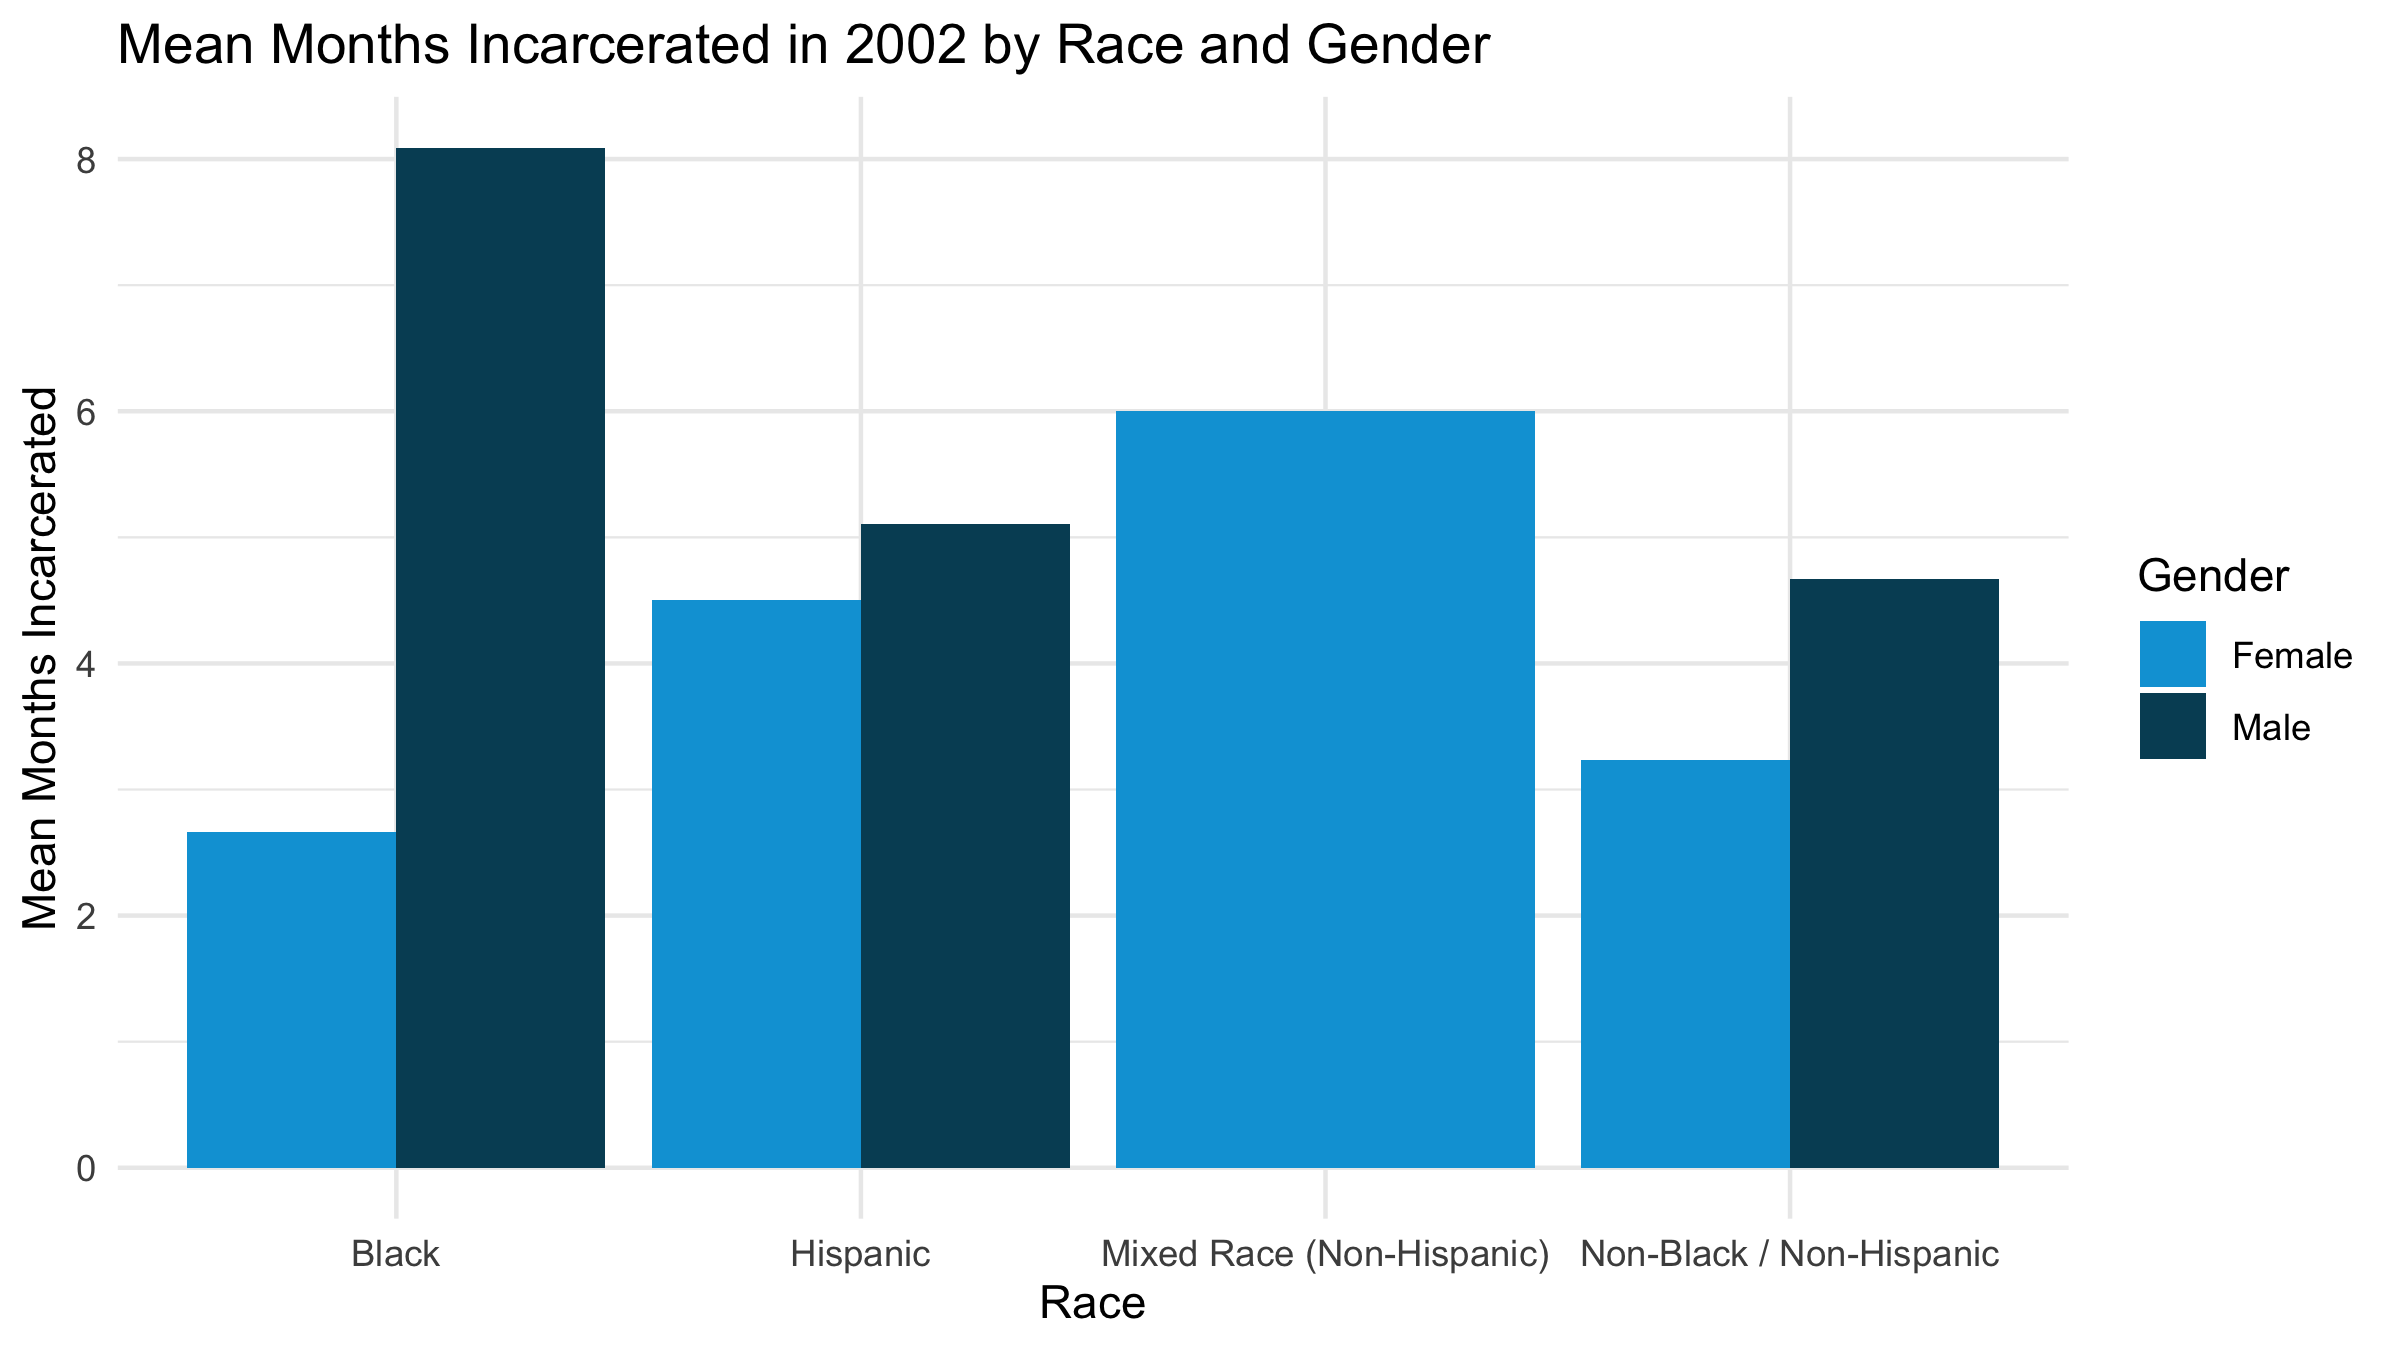
\includegraphics[width=.85\textwidth]{incarcerations_by_racegender}
    \end{center}
    \caption{Mean Months Incarcerated in 2002 by Race and Gender}
\end{figure}

\begin{table}[H]

\caption{\label{tab:tab:summarystats}Mean Months Incarcerated in 2002 by Race and Gender}
\centering
\begin{tabular}[t]{lrrrr}
\toprule
Gender & Black & Hispanic & Mixed Race Non Hispanic & Non Black Non Hispanic\\
\midrule
\cellcolor{gray!6}{Female} & \cellcolor{gray!6}{2.666667} & \cellcolor{gray!6}{4.500000} & \cellcolor{gray!6}{6} & \cellcolor{gray!6}{3.230769}\\
Male & 8.090909 & 5.103448 & NA & 4.666667\\
\bottomrule
\end{tabular}
\end{table}

\newpage

In Table 2 below, we can see the results from the regression model. Hispanic Females are estimated to be incarcerated about 2.3 months shorter than Black Females, and Non-Black/Non-Hispanic Females are estimated to be incarcerated about 2.9 months shorter than Black Females. However, Mixed Race (Non-Hispanic) Females are estimated to be incarcerate about 0.9 months longer than Black Females. 
Meanwhile, the only Non-Black male group that is estimated to be incarcerated longer than Black Females are Hispanic Males, who are estimated to be incarcerated about 0.3 months longer than Black Females. 


% Table created by stargazer v.5.2.2 by Marek Hlavac, Harvard University. E-mail: hlavac at fas.harvard.edu
% Date and time: Thu, Feb 17, 2022 - 15:01:39
\begin{table}[!htbp] \centering 
  \caption{Regression Output. Omitted category is Black Females.} 
  \label{tab:regression} 
\begin{tabular}{@{\extracolsep{5pt}}lc} 
\\[-1.8ex]\hline 
\hline \\[-1.8ex] 
 & \multicolumn{1}{c}{\textit{Dependent variable:}} \\ 
\cline{2-2} 
\\[-1.8ex] & Months Incarcerated in 2002 \\ 
\hline \\[-1.8ex] 
 Hispanic & $-$0.159$^{***}$ \\ 
  & (0.038) \\ 
  & \\ 
 Mixed Race (Non-Hispanic) & $-$0.174$^{**}$ \\ 
  & (0.083) \\ 
  & \\ 
 Non-Black / Non-Hispanic & $-$0.189$^{***}$ \\ 
  & (0.035) \\ 
  & \\ 
 Male & 0.194$^{***}$ \\ 
  & (0.022) \\ 
  & \\ 
 Constant & 0.155$^{***}$ \\ 
  & (0.026) \\ 
  & \\ 
\hline \\[-1.8ex] 
Observations & 8,621 \\ 
R$^{2}$ & 0.015 \\ 
Adjusted R$^{2}$ & 0.014 \\ 
Residual Std. Error & 1.019 (df = 8616) \\ 
F Statistic & 32.033$^{***}$ (df = 4; 8616) \\ 
\hline 
\hline \\[-1.8ex] 
\textit{Note:}  & \multicolumn{1}{r}{$^{*}$p$<$0.1; $^{**}$p$<$0.05; $^{***}$p$<$0.01} \\ 
\end{tabular} 
\end{table} 


\newpage

\section{Conclusion}

Figure 1 provides some preliminary evidence of a significant relationship between incarceration, race, and gender. However, the estimated regression results say otherwise. While the regression coefficients are large in magnitude, none of the coefficients are statistically significant at the 90 percent level. 
Therefore, the model provides no estimate of a statistically significant relationship, so there is no statistical evidence that race and gender affect incarceration. 

However, the results of this model may be due to the limited sample size of the dataset. If this anlysis were to be replicated with data aggregated over several years, we could increase the sample size and accuracy of our estimates. Moreover, we could guarantee observations for every group, because this sample had no incarcerated individuals in the Mixed Race (Non-Hispanic) Male group, which likely limited the accuracy of the results. 
While this analysis is limited in its effectiveness in estimating incarceration by race and gender, it does suggest that a statistically significant relationship could potentially be found in a larger more balanced sample. 

\end{document}
